% VUT FIT MITAI
% MSZ 2021/2022
% Author: Vladimir Dusek
% Login: xdusek27

%%%%%%%%%%%%%%%%%%%%%%%%%%%%%%%%%%%%%%%%%%%%%%%%%%%%%%%%%%%%%%%%%%%%%%%%%%%%%%%%

% Path to figures
\graphicspath{{upa/prostorove_db_indexace/figures}}

%%%%%%%%%%%%%%%%%%%%%%%%%%%%%%%%%%%%%%%%%%%%%%%%%%%%%%%%%%%%%%%%%%%%%%%%%%%%%%%%

\chapter{UPA~--~Indexace (nejen) v prostorových DB (kD-Tree a Grid File (a jejich varianty), R-Tree).}

%%%%%%%%%%%%%%%%%%%%%%%%%%%%%%%%%%%%%%%%%%%%%%%%%%%%%%%%%%%%%%%%%%%%%%%%%%%%%%%%

\section{Zdroje}

\begin{compactitem}
    \item \path{PDB-Spatial-CZ.pdf}
    \item \path{03-spatial_databases.pdf}
    \item \path{szz-kastak.pdf}
    \item \path{szz-discord-bazi.pdf}
\end{compactitem}

%%%%%%%%%%%%%%%%%%%%%%%%%%%%%%%%%%%%%%%%%%%%%%%%%%%%%%%%%%%%%%%%%%%%%%%%%%%%%%%%

\section{Úvod a kontext}

\begin{compactitem}
    \item Ve vícedimenzionálním prostoru nelze z reprezentace hodnot jednoznačně určit uspořádání -- předchůdce a následníka. Nelze tedy použít obecně užívané indexační algoritmy pro 1D.

    \item Řešení v podobě mapování do 1D nám většinou nestačí, proto se v prostorových databázích využívají specializované indexační algoritmy.
\end{compactitem}

%%%%%%%%%%%%%%%%%%%%%%%%%%%%%%%%%%%%%%%%%%%%%%%%%%%%%%%%%%%%%%%%%%%%%%%%%%%%%%%%

\section{Mapování do 1D}

\begin{compactitem}
    \item Nejjednodušší řešení je namapovat data do jednorozměrného prostoru.
    \item Touto transformací však zcela jistě ztratíme sousednost.
    \item Krom toho, taková transformace nemusí být vůbec realizovatelná. A pokud ano, tak výsledek dotazů nemusí být transformovatelný zpět, takže lze výsledek jen těžko interpretovat.
\end{compactitem}

%%%%%%%%%%%%%%%%%%%%%%%%%%%%%%%%%%%%%%%%%%%%%%%%%%%%%%%%%%%%%%%%%%%%%%%%%%%%%%%%

\section{Indexace bodů}

\begin{compactitem}
    \item Pro indexaci bodů využíváme 2 přístupy: stromy dělící prostor a hashování.
\end{compactitem}

\subsection{Stromy dělící prostor}

\begin{compactitem}
    \item Myšlenka: vytvoříme uspořádání na množině bodů v prostoru (podobně jako ho máme přirozeně na množině čísel) a díky tomu, budeme moct uspořádat body do stromu.
\end{compactitem}

\subsubsection{k-D Tree}

\begin{compactitem}
    \item k-D Tree je datová struktura (binární strom) dělící prostor hyperplochami na nejvyšší možné úrovni, a to vždy na dvě části. \begin{compactitem}
        \item Hyperplocha v rovině je přímka.
        \item Dělící hyperplocha musí být rovnoběžná s osovým (souřadným) systémem.
        \item Při dělení, musí ve výsledných plochách být obsažen vždy aspoň jeden bod, který pak už není součástí jakékoli jiné hyperplochy.
    \end{compactitem}

    \item Implementace stromu: \begin{compactitem}
        \item vytvoření stromu -- pomocí rekurze;
        \item vyhledávání -- bez problému, cyklus;
        \item vkládání -- pomocí rekurze (pořadí vkládání bodů výrazně ovlivňuje vyváženost výsledného stromu);
        \item mazání -- velký problém, vyžaduje znovuvložené celého podstromu.
    \end{compactitem}

    \item Závěr: díky problematica mazání uzlů se tato struktura používá pouze pro pro statická data.
\end{compactitem}

\begin{figure}[H]
    \centering
    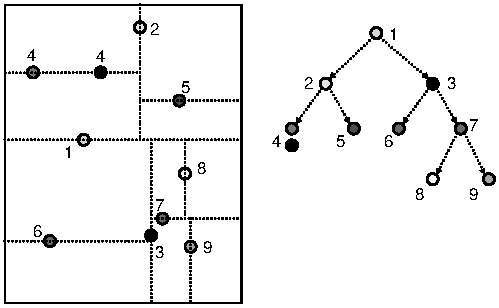
\includegraphics[width=0.75\linewidth]{kd_tree.pdf}
    \caption{Příklad k-D Tree. Pořadí vkládání uzlů do indexačního stromu probíhalo podle číslovek u uzlu.}
\end{figure}

\subsubsection{Adaptivní k-D Tree}

\begin{compactitem}
    \item Snaží se eliminovat problémy spojené s pořadím vkládání bodů.

    \item Shodný s k-D Tree, až na to, že dělící hyperplochy
    \begin{compactitem}
        \item už nemusí obsahovat nějaký bod, stačí, že dělí prostor;
        \item jsou vybírány tak, aby výsledný prostor obsahoval přibližně stejný počet bodů.
    \end{compactitem}

    \item Ze změn vyplývá, že data jsou uložena až v listových uzlech.

    \item Závěr: vylepšeno vkládání, ale mazání je stále velký problém, proto vhodnost stále spíše pro statická data.
\end{compactitem}

\begin{figure}[H]
    \centering
    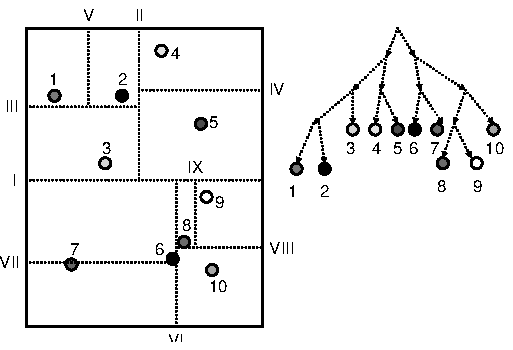
\includegraphics[width=0.75\linewidth]{adaptivni_kd_tree.pdf}
    \caption{Příklad Adaptivního k-D Tree. Římská čísla označují pořadí dělení prostoru.}
\end{figure}

\subsubsection{BSP (\textit{binary space partitioning}) Tree}

\begin{compactitem}
    \item Stejný jako Adaptivní k-D Tree až na to, že dělící hyperplochy nemusí být rovnoběžné s osovým (souřadným) systémem.
    \item Prostor se dělí do doby, než počet bodů v ploše neklesne pod určitou hodnotu (na obrázku 2).
    \item Algoritmus není adaptivní (odolný proti změně dat).
    \item Má vyšší nároky na paměť než k-D Tree, u kterého šlo díky pravidelnému střídání dělení ignorovat jednu souřadnici hyperplochy.
\end{compactitem}

\begin{figure}[H]
    \centering
    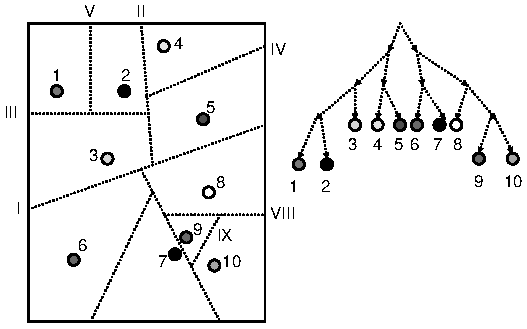
\includegraphics[width=0.75\linewidth]{bsp_tree.pdf}
    \caption{Příklad BSP Tree. Římská čísla označují pořadí dělení prostoru.}
\end{figure}

\subsubsection{Quad Tree}

\begin{compactitem}
    \item Algoritmus, který se plně shoduje s K-D Tree, avšak s rozdílem, že nedělí prostor na polovinu, ale na $2^n$ podstromů ($n$ je stupeň dimenze prostoru). \begin{compactitem}
        \item Díky tomu nemusejí být podstromy shodné, neboť některé listy nemusejí vést do míst, kde je obsažen nějaký bod.
    \end{compactitem}
    \item Prostor se dělí do doby, než počet bodů v ploše neklesne pod určitou hodnotu (na obrázku 2).
    \item Některé prostory neobsahují žádný bod.
\end{compactitem}

\begin{figure}[H]
    \centering
    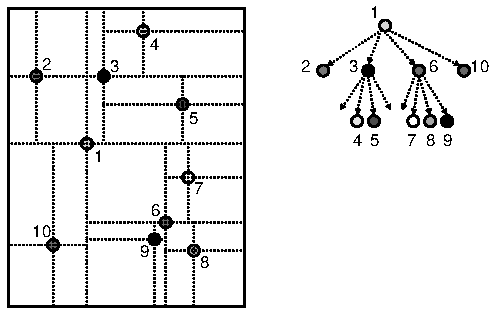
\includegraphics[width=0.75\linewidth]{quad_tree.pdf}
    \caption{Příklad Quad Tree. Čísla u bodů označují pořadí, v jakém je prostor dělen hyperplochami na $2^n = 4$ podprostory a jak jsou vkládány údaje do stromu. Některé větve nemusejí obsahovat data, i když sousední je obsahují.}
\end{figure}

\subsection{Hashování}

\begin{compactitem}
    \item Tzv. adaptivní a lineární hashování \todo{?}.
\end{compactitem}

\subsubsection{Grid File}

\begin{compactitem}
    \item Sledovaný úsek prostoru je rozdělen $n$-rozměrnou mřížkou (ne nutně pravidelnou) na buňky. \begin{compactitem}
        \item Buňky obsahují různý počet bodů, klidně 0.
    \end{compactitem}

    \item K tomuto základnímu rozdělení existuje adresář, který každou buňku přiřazuje k datové jednotce. (\textit{bucket}). \begin{compactitem}
        \item Adresář je poměrně velký, proto je vždy ukládán na disk.
        \item Mřížka je také uložena na disku, nicméne pro vyhledání datové jednotky stačí 2 přístupy na disk, což je snesitelné.
    \end{compactitem}

    \item Při vkládání může dojít k přetečení (datová jednotka není schopna pojmout další údaj), které není lokální. \begin{compactitem}
        \item Je nutné vložit rozdělující hyperplochu a tak zvětšit adresář.
        \item Podobně se chová i mazání -- jelikož není lokální, tak odstranění hyperplochy je třeba prověřit. Pokud je dat málo, tak může zaniknout i datová jednotka (data buďto zanikla s ní, nebo jsou přesunuta do jiné datové jednotky).
    \end{compactitem}
\end{compactitem}

\begin{figure}[H]
    \centering
    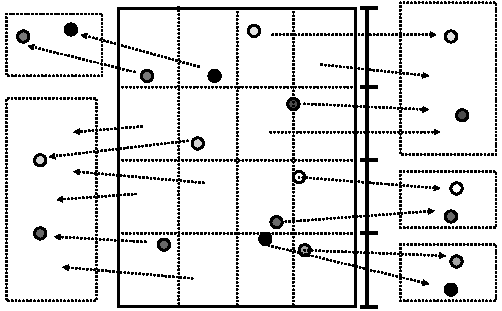
\includegraphics[width=0.75\linewidth]{grid_file.pdf}
    \caption{Příklad Grid File.}
\end{figure}

\subsubsection{Two-level Grid File}

\begin{compactitem}
    \item Je zavedena mřížka druhé úrovně. \begin{compactitem}
        \item Vzniká vztah kořenový adresář a podadresář.
        \item První úroveň slouží pouze jako ukazatel do základní struktury Grid filu.
    \end{compactitem}

    \item V takovém systému jsou změny při vkládání či mazání často lokální, nicméně i tak není problematika přetečení úplně vyřešena.

    \item Na nejvyšší úrovni dělí mřížka oblast na poměrně velké celky. Tyto velké celky jsou poté předmětem delení autonomní struktury Grid File. Jedná se tedy o dvě úrovně, kde ta první odkazuje pouze na základní strukturu Grid File a až ta odkazuje na datové jednotky.
\end{compactitem}

\begin{figure}[H]
    \centering
    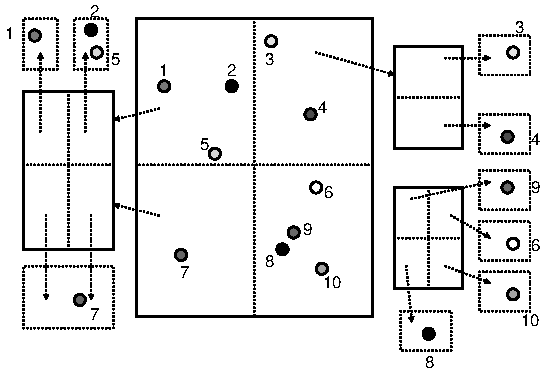
\includegraphics[width=0.75\linewidth]{grid_file_two_level.pdf}
    \caption{Příklad Two-level Grid File.}
\end{figure}

\subsubsection{Twin Grid File}

\begin{compactitem}
    \item Celá struktura Grid File se vyskytuje dvakrát. \begin{compactitem}
        \item Není však v hierarchickém (vertikálním) vztahu (jako u Two Level) ale v horizontálním.
        \item I když je jedna ze struktur nadřazená, tak je jedno, která to bude.
    \end{compactitem}
    \item Cílem je maximálně využít prostor pro indexovací strukturu. \begin{compactitem}
        \item Data se mezi obě části dělí prakticky rovnoměrně.
        \item Jedna struktura je však primární a druhá je sekundární (přetoková).
    \end{compactitem}
    \item Algoritmus umožňuje úplnou paralelizaci vyhledávání a částečnou pro vkládání.
\end{compactitem}

\begin{figure}[H]
    \centering
    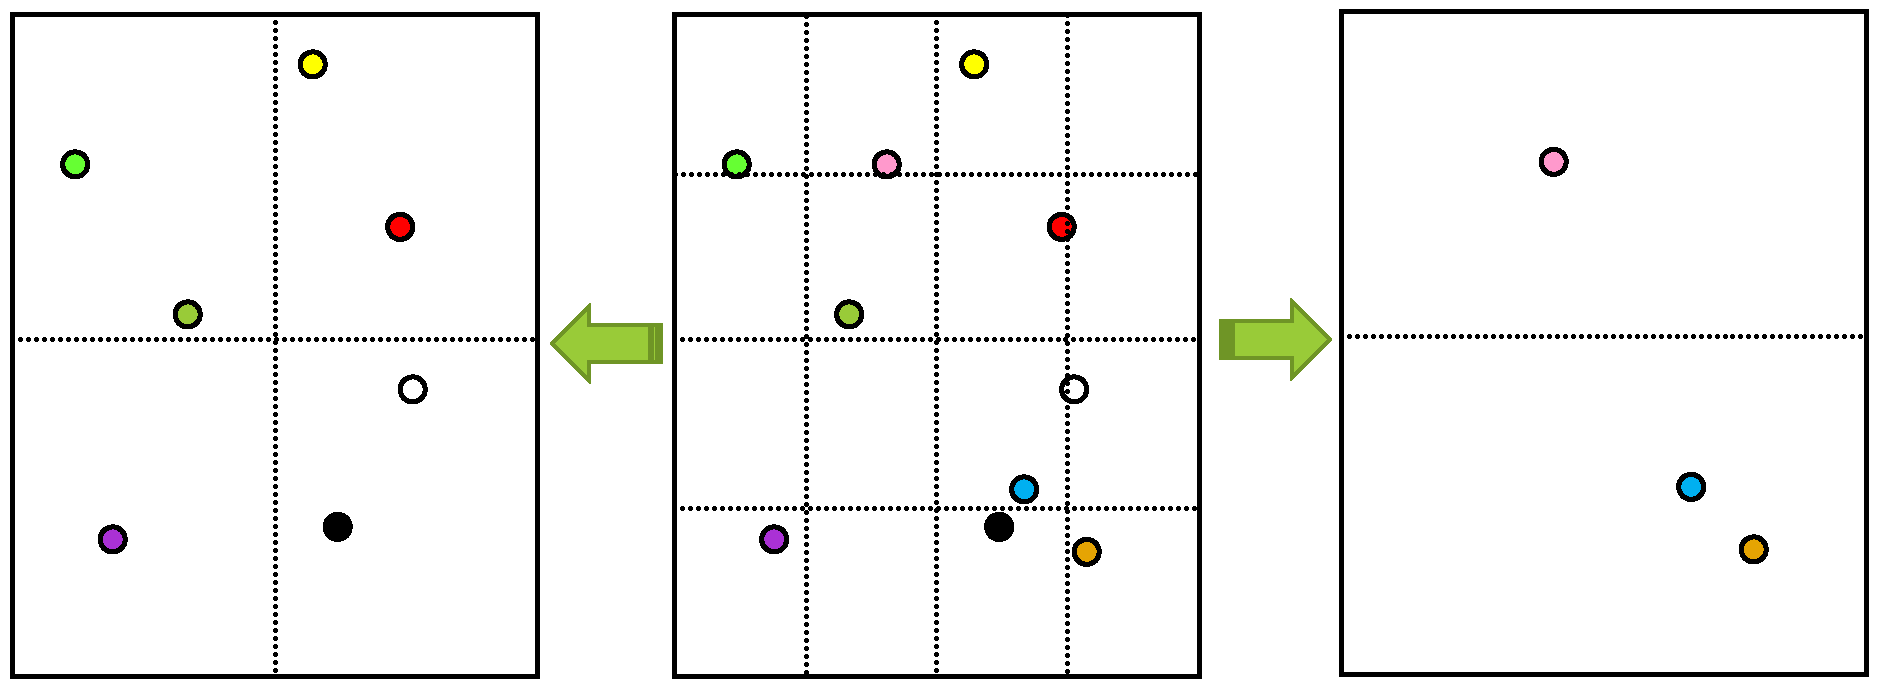
\includegraphics[width=0.9\linewidth]{grid_file_twin.pdf}
    \caption{Příklad Twin Grid File (1).}
\end{figure}

\begin{figure}[H]
    \centering
    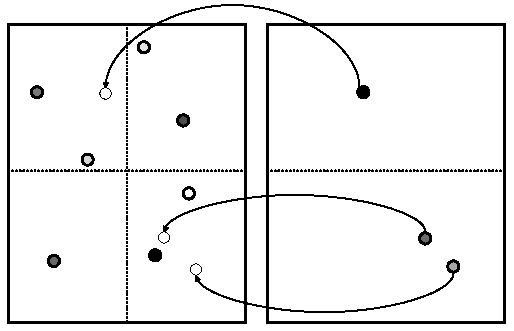
\includegraphics[width=0.9\linewidth]{grid_file_twin_2.pdf}
    \caption{Příklad Twin Grid File (2). Na obrázku je ukázáno jak jsou do přetokové struktury odkládány body tak, aby nedošlo k přetečení ve struktuře primární. Šipky naznačují umístění bodů v prostoru. Do sekundární struktury (pravé) se body přesouvají tehdy, pokud by mělo dojít k rozdělení primární struktury a přitom úroveň sekundární struktury je menší, nebo je schopna bod pojmout bez dělení.}
\end{figure}

%%%%%%%%%%%%%%%%%%%%%%%%%%%%%%%%%%%%%%%%%%%%%%%%%%%%%%%%%%%%%%%%%%%%%%%%%%%%%%%%

\section{Indexace vícerozměrných objektů}

\begin{compactitem}
    \item Uložení bodů je sice primární, ale v obecné realitě s ním nelze vystačit, proto vznikly algoritmy pro indexaci vícerozměrných útvarů, které používají buďto překrývání (\textit{overlapping}) a nebo ořezávání (\textit{clipping}).
\end{compactitem}

\subsection{Překrývání -- R-Trees}

\begin{compactitem}
    \item Indexační struktury se překrývají, takže vzniká více vyhledávacích cest, implementačně se buňky překrývají svými hranicemi.

    \item V praxi tak dochází k tomu, že algoritmus je stejný, jen počet prohledávacích cest se zvětšuje, protože dopředu není jasné, ve které buňce je nakonec objekt uložen.
\end{compactitem}

\begin{figure}[H]
    \centering
    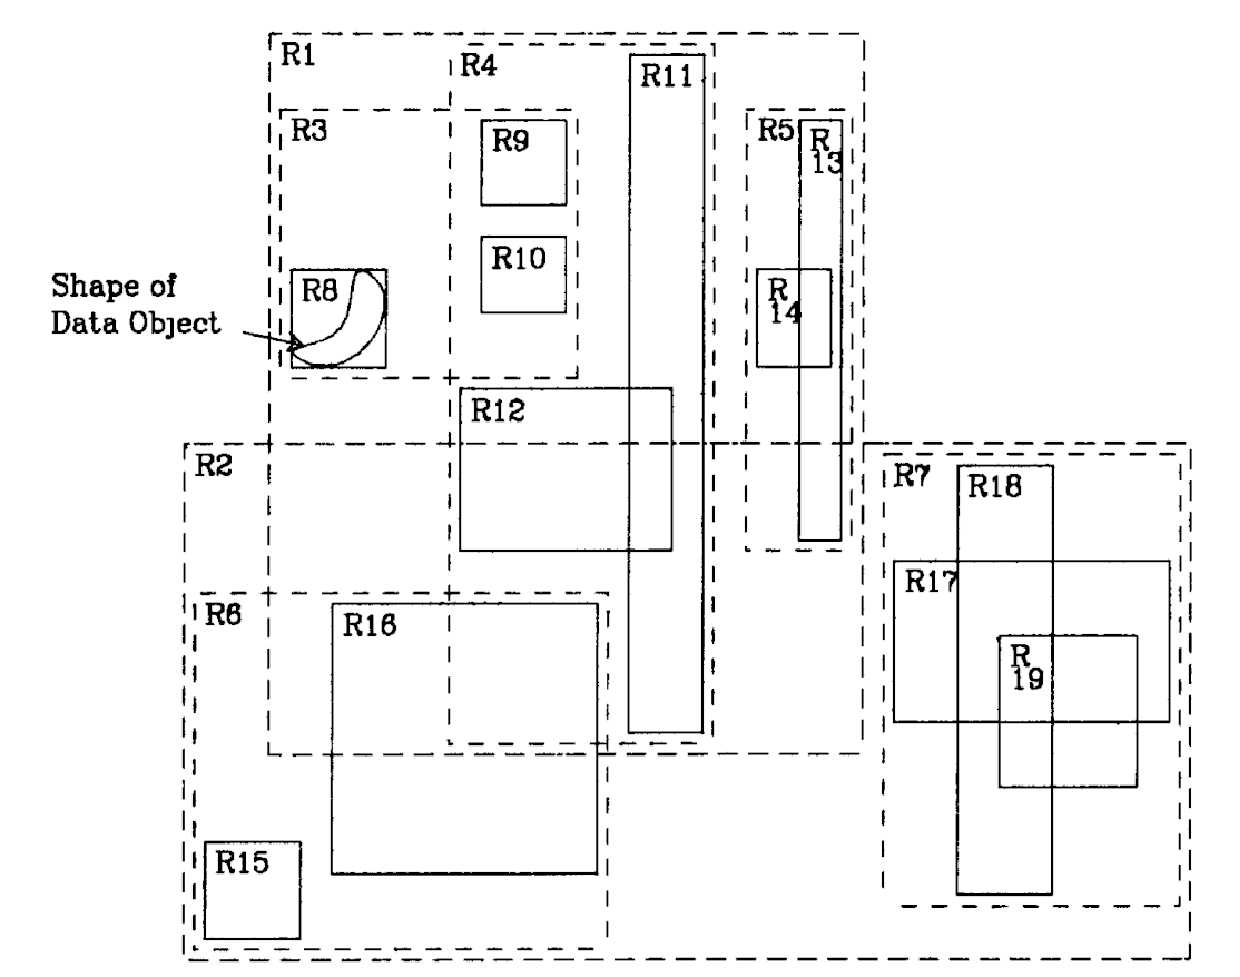
\includegraphics[width=0.85\linewidth]{r_tree_1.pdf}
    \caption{R-Tree příklad.}
\end{figure}

\begin{figure}[H]
    \centering
    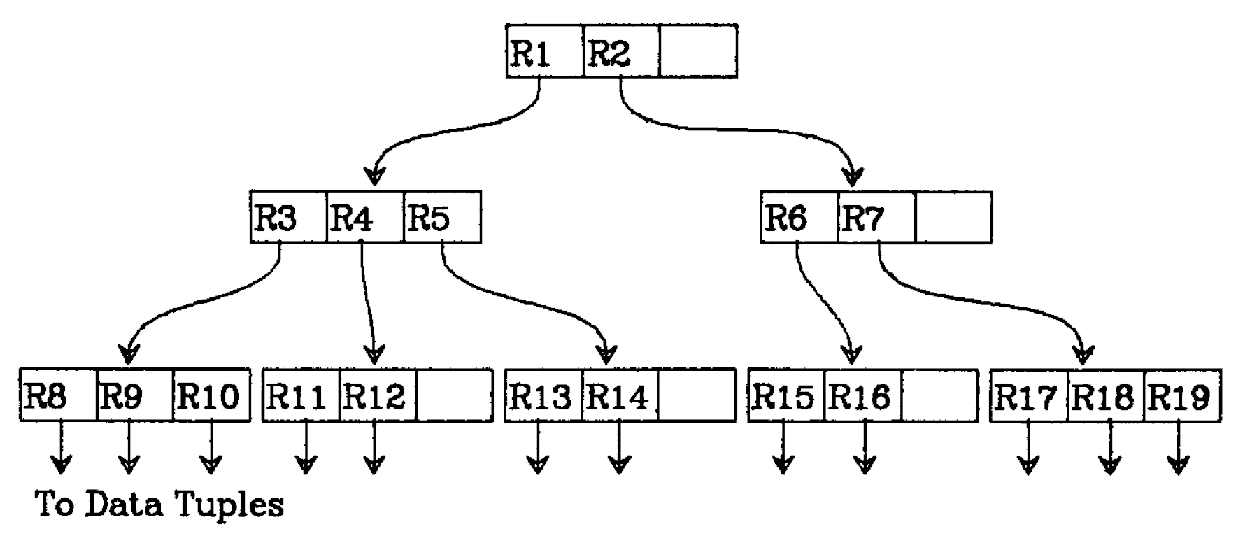
\includegraphics[width=0.85\linewidth]{r_tree_2.pdf}
    \caption{R-Tree příklad -- index.}
\end{figure}

\subsection{Ořezávání -- $\text{R}^+$-Trees}

\begin{compactitem}
    \item U metod založených na ořezávání není povoleno, aby se MBB (\textit{minimal bounding box}), buňky překrývaly.
    \item Jediným řešením je rozsekat objekty tak, aby sledovaly hranice dělicích MBB. Jeden objekt tak může být rozdělen na více.
    \item Při vyhledávání pak tedy nestačí vyhledat objekt, ale je třeba se vrátit k jeho původní, nedělené reprezentaci.
\end{compactitem}

\begin{figure}[H]
    \centering
    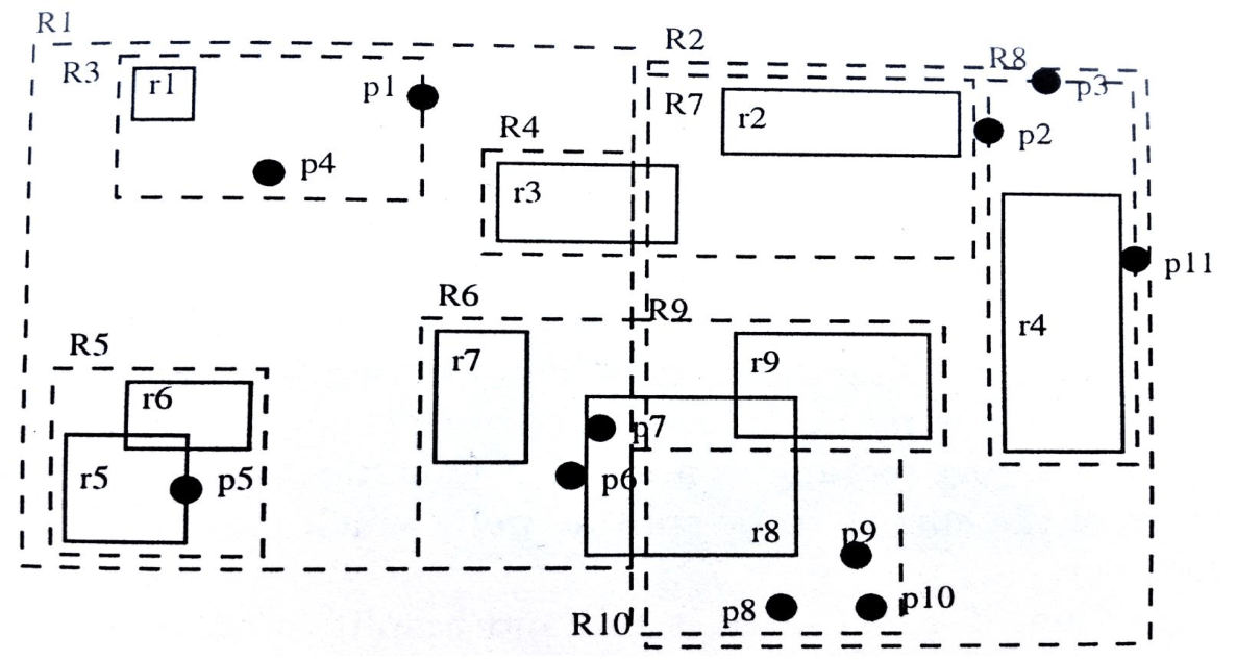
\includegraphics[width=0.85\linewidth]{r_tree_plus_1.pdf}
    \caption{$\text{R}^+$-Tree příklad.}
\end{figure}

\begin{figure}[H]
    \centering
    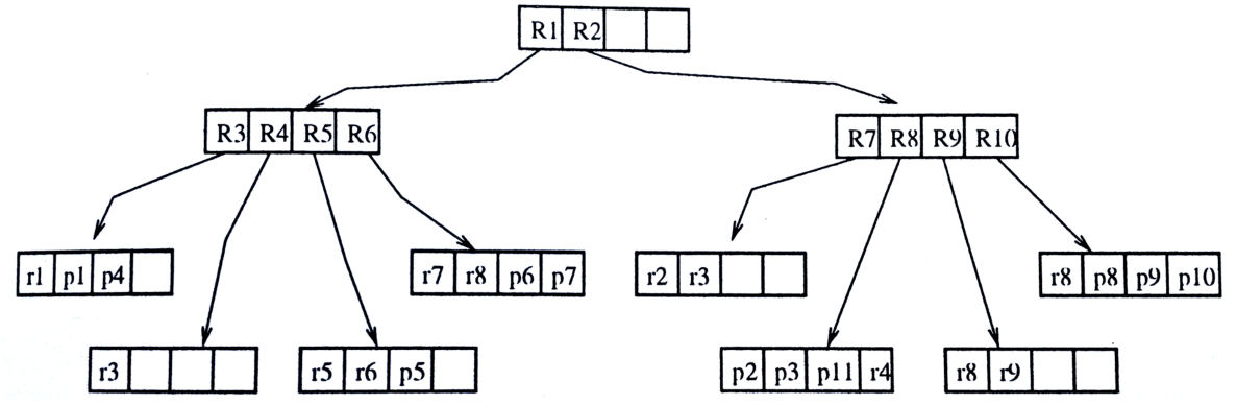
\includegraphics[width=1\linewidth]{r_tree_plus_2.pdf}
    \caption{$\text{R}^+$-Tree příklad -- index.}
\end{figure}
